\documentclass{scrartcl}
\usepackage[utf8]{inputenc}
\usepackage{hyperref}
\usepackage{graphicx}
\usepackage{amsmath}
\setkomafont{disposition}{\normalfont\bfseries}
\begin{document}
\title{STA6166 Final Project}
\author{Biswas, Sayak}
\subtitle{Final Project Report for STA6166\\Spring 2017}
\maketitle
\section{PSA Level Modeling}
\subsection{Introduction}
\par
The problem is to model the prostate-specific antigen(PSA) with respect to some clinical measurements. The provided number of data points in the sample is 97. I calculated some descriptive statistics on the sample provided. The mean PSA level of the sample is 23.73 mg/ml with a standard deviation of 40.78 mg/ml and a median value of 13.33 mg/ml.
\par
Since we are to model PSA Level, we take it as the response variable and the rest as the variables as the predictors. To get an initial idea about the kind of relationship PSA Level has with the other variables we plot scatter graphs. Unfortunately, with this data set te scatterplots don't quite paint a clear picture of the relationship between the variables except \textit{PSA Level vs. Cancer Volume} which seems to present a slight positive relationship. So, next we create a correlation matrix of the various variables. We can see that there is a moderately positive correlation between \textit{Cancer Volume} and \textit{Capsular Penetration}.
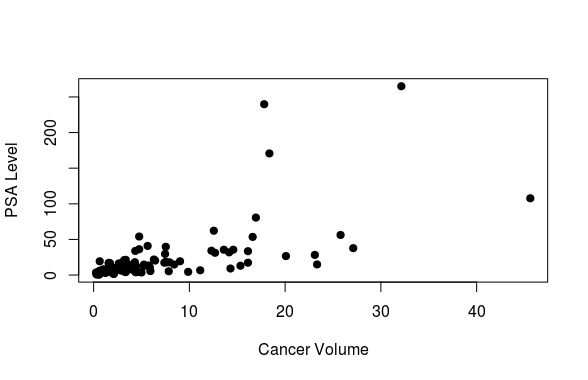
\includegraphics[width=0.4\textwidth]{psa_cancervol.png}
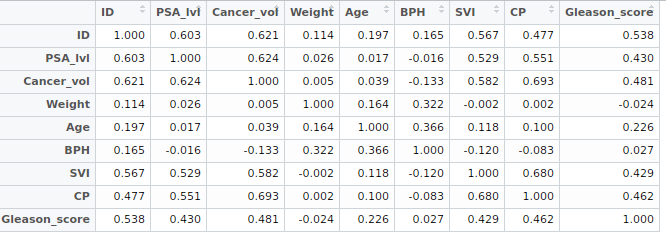
\includegraphics[width=0.4\textwidth]{Correlation_Matrix.png}
\par
Keeping the previous observations in mind, we now develop a full linear model using all the predictors and without any interaction terms. Assuming all the model assumptions are met(we will verify this later), we test the overall fit of the model with the below hypotheses:\\
\begin{center}
$H_0: \beta_1=...=\beta_7=0$ vs $H_a: \text{at least one of them} \neq 0$\\
\end{center}
This initial model has $R^2 = 45.85\%$ and ${R^2}_{adj} = 41.59\%$. This means that this model is able to explain a large portion of the variability. Also the test statistic value is $T.S. = 10.77$ with an associated p-value of almost 0 found using an $F_{7,39}$ distribution. So, at least one predictor is significant. We will use this information to check if the model can be reduced in any way as the AIC value is around 952.17.
\par For now let's validate if the model assumptions are met. We make use of the automated \textit{check} function provided by the professor. The graphs generated are shown below:\\
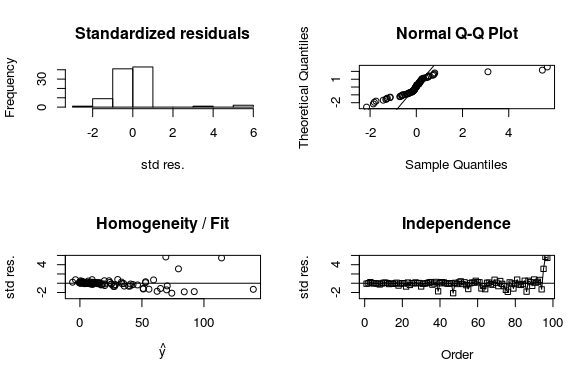
\includegraphics[width=\textwidth]{psa_check.png}\\ 
\begin{itemize}
  \item We can see that the QQ plot and the histogram show heavier left and right tails compared to the normal. Also, the Shapiro-Wilk test which gives a p-value of almost 0 and hence confirms violation of normality. 
  \item As there is no discernible pattern in the time-series plot of the data, we can safely conclude the data to be independent.
  \item From the graph, variance doesn't seem to constant at all places but the fit of the model seems to be almost correct.
\end{itemize}
In light of the above, we perform Box-Cox transformation which fixes the violations as can be seen below:\\
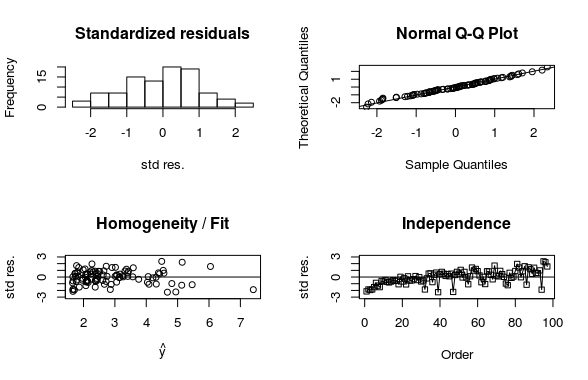
\includegraphics[width=\textwidth]{psa_transform_check.png}\\
Now, we perform automatic reduction of model using the stepT function provided to us. This removes the predictors with high p-values and the ones which are highly correlated. Thus \textit{Age}, \textit{Weight} and \textit{Capsular Penetration} are removed. We now see that the $R_2$ has increase to 60.71\% and ${R^2}_{adj} = 59\%$. Also, the AIC value has reduced to 273.99.
\par
We still haven't addressed the fact that we have a qualitative predictor i.e. \textit{Seminal vesicle invasion}. So, we use scatterplots with regression line enabled to check for interaction between this and the other variables.\\
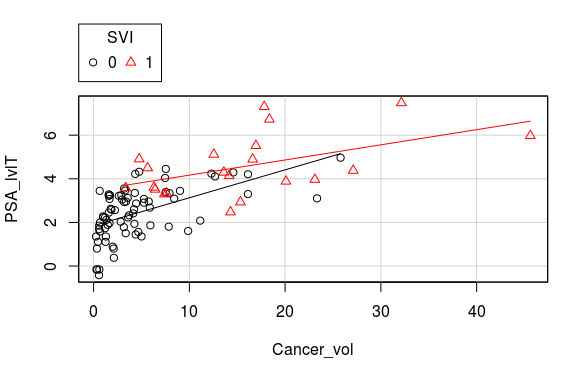
\includegraphics[width=0.3\textwidth]{svi_cancervol.png}
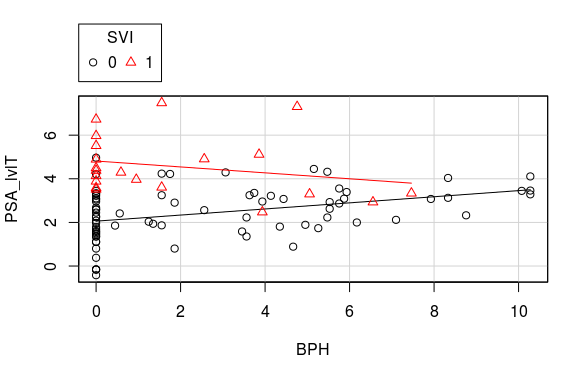
\includegraphics[width=0.3\textwidth]{svi_bph.png}
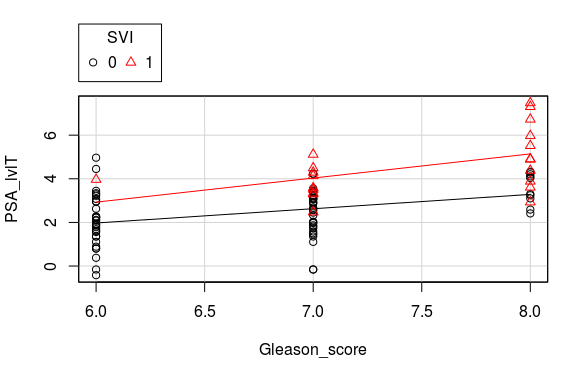
\includegraphics[width=0.3\textwidth]{svi_gscore.png}
\end{document}
